\documentclass[mathserif,professionalfont]{beamer}
\usepackage{pxfonts} 
%\usepackage{eulervm}
\usepackage[english]{babel}
\usepackage{calc}
\usepackage[absolute,overlay]{textpos}
\mode<presentation>{\usetheme{tud}}
%\usepackage{subcaption}
\usepackage{tcolorbox}
\usepackage{tikz}
\usetikzlibrary{positioning,arrows}
\usepackage[utf8x]{inputenc}
\usepackage{scalefnt}
\usetikzlibrary{decorations.markings}
\usetikzlibrary{shapes,snakes}
\usetikzlibrary{shapes.geometric}
\usetikzlibrary{fit}					
\usetikzlibrary{backgrounds}
\usetikzlibrary{positioning}
\usetikzlibrary{arrows}
\usepackage{pgffor}
\usepackage{amsmath,amssymb,mathrsfs}
\usepackage{amsthm}
\usepackage{color}
\usepackage{wasysym}
\usepackage{pdfpages}
\usepackage{paralist}
\usepackage{framed}
\usepackage{fancybox} %kaders
\usepackage{pifont}
\usepackage{pgfplots}
\usepackage{listofsymbols}
\usepackage{multirow}
%\usepackage[pdftex]{hyperref}
%\usepackage{enumitem}
\tikzstyle{every picture}+=[remember picture]
\tikzstyle{na} = [baseline=-.5ex]


\title[Accuracy of original MPM]{Accuracy of original MPM}
%\institute[]{}
\author[]{Lisa Wobbes, Roel Tielen}
\date[\today]{\today}

\definecolor{blueM}{rgb}{0.4, 0.6, 0.8}

\begin{document}
%titel----------------------------------------------------------------------------------------------------------------------------------------------------------------
{
%\usebackgroundtemplate{\includegraphics[width=\paperwidth,height=\paperheight]{logos}}%
%\setbeamertemplate{footline}{\usebeamertemplate*{minimal footline}}
\frame{\titlepage}
}

%outline------------------------------------------------------------------------------------------------------------------------------------------------------------
\begin{frame}{Outline}
\begin{itemize}
\item Numerical accuracy
\item Benchmarks
	\begin{itemize}
	\item Vibrating bar 
	%\item Vibrating hyper-elastic bar
	\item Oedometer
	\end{itemize}
\item
\item
\item
\end{itemize}
\end{frame}

%------------------------------------------------------------------------------------------------------------------
\begin{frame}{Numerical accuracy}
\begin{tcolorbox}[colback=red!5,colframe=red!50!black,title=Numerical Approximation]
$u_{ex} = u_{num} + \mathcal{O}(\Delta x^n) + \mathcal{O}(\Delta t)$ %with $n \leq 2$
\end{tcolorbox}
\begin{tcolorbox}[colback=red!5,colframe=red!50!black,title=RMS Error]
$Error_{RMS} = \sqrt{\frac{1}{n_p} \left(\sum_{p=1}^{n_p}u_{num}(x_p,t) - u_{ex}(x_p,t)\right)^2}$
\end{tcolorbox}
\begin{tcolorbox}[colback=blue!5,colframe=blue!40!black,title=Accuracy in displacement]
For $\Delta t \to 0$, the order of accuracy is equal to $n$, i.e. the reduction of $\Delta x$ by a factor of 2 decreases the RMS error by $2^n$.
\end{tcolorbox}
\end{frame}

%------------------------------------------------------------------------------------------------------------------
\begin{frame}{Vibrating bar}
  \begin{minipage}{\linewidth}
      \centering
      \begin{minipage}{0.45\linewidth}
              \definecolor{darkred}{cmyk}{0,0.9,0.9,0.2}
\definecolor{darkblue}{cmyk}{0.9,0.5,0.1,0.2}
\tikzset{
mystyle1/.style={
  rectangle,
  inner sep=0.05pt,
  text width=1mm,
  fill=black
  }
}

\tikzset{
mystyle2/.style={
  circle,
  inner sep=0.1pt,
  text width=2mm,
  fill=red!80
  }
}
\tikzstyle{myarrows}=[line width=0.4mm,draw=darkred,postaction={draw, line width=0.4mm, shorten >=3mm, -}]
\begin{figure}[H]
\centering
\begin{tikzpicture}[scale=0.48]
 %structure
 \draw[fill=black!25] (0.5,2) rectangle (6.5,2.55);
 \draw[fill=darkblue] (-0.3,3.5) rectangle (0.5,1);
%initial velocity
\foreach \i in {1,...,5}
{
        \pgfmathsetmacro{\z}{0.5 + (6/5)*\i};
        \pgfmathsetmacro{\y}{2.275};
        \pgfmathsetmacro{\l}{1.5*sin((175*\z)/12)};
        \draw[myarrows] (\z,\y) -- (\z,\y+\l);
	\draw[->, ultra thick,darkred] (\z,\y+1.01*\l) -- (\z,\y+1.05*\l);
}
\draw (7.2,3.2) node {$v_0$};
%coordinate
\draw[->, thick] (-0.3,0.2)--(7.8,0.2);
\draw (7.5, -0.4) node {$x$};
 %coordinates
 \draw[thick] (0.5, 0.05)--(0.5,0.35);
 \draw (0.5,-0.4) node {0};
 \draw[thick] (6.5, 0.05)--(6.5,0.35);
 \draw (6.5,-0.4) node {$L$};
\end{tikzpicture}
\end{figure}
      \end{minipage}
      \hspace{0.01\linewidth}
      \begin{minipage}{0.45\linewidth}
         \begin{align}\nonumber
&\frac{\partial^2 u}{\partial t^2} = \frac{E}{\rho}\frac{\partial^2 u}{\partial x^2} \\ \nonumber
&\mbox{Boundary conditions: } \\  \nonumber
& u(0,t) = 0\\ \nonumber
& \frac{\partial u}{\partial x}(L,t) = 0\\  \nonumber
&\mbox{Initial conditions:}\\  \nonumber
& u(x,0) = 0\\ \nonumber
& \frac{\partial u}{\partial t}(x,0) = v_0\sin \left( \frac{\pi x}{2L} \right)
\end{align} 
      \end{minipage}
  \end{minipage}
\end{frame}

%%------------------------------------------------------------------------------------------------------------------
%\begin{frame}{Vibrating hyper-elastic bar}
%  \begin{minipage}{\linewidth}
%      \centering
%      \begin{minipage}{0.45\linewidth}
%\definecolor{darkred}{cmyk}{0,0.9,0.9,0.2}
%\definecolor{darkblue}{cmyk}{0.9,0.5,0.1,0.2}
%\tikzset{
%mystyle1/.style={
%  rectangle,
%  inner sep=0.05pt,
%  text width=1mm,
%  fill=black
%  }
%}
%
%\tikzset{
%mystyle2/.style={
%  circle,
%  inner sep=0.1pt,
%  text width=2mm,
%  fill=red!80
%  }
%}
%\tikzstyle{myarrows}=[line width=0.4mm,draw=darkred,postaction={draw, line width=0.4mm, shorten >=3mm, -}]
%\begin{figure}[h]
%\centering
%\begin{tikzpicture}[scale = 0.48]
%%structure
% \draw[fill=black!25] (0.5,2) rectangle (6.5,2.55);
% \draw[fill=darkblue] (-0.3,3.5) rectangle (0.5,1);
%%traction force	
%\draw[->, ultra thick,darkred] (6.5,3.2) -- (8.2,3.2);
% \draw (7.15,3.9) node {$F_{trac}$};
%%coordinate
%\draw[->, thick] (-0.3,0.4)--(8.2,0.4);
%\draw (7.9, -0.7) node {$x$};
% %coordinates
% \draw[thick] (0.5, 0.05)--(0.5,0.35);
% \draw (0.5,-0.4) node {0};
% \draw[thick] (6.5, 0.05)--(6.5,0.35);
% \draw (6.5,-0.4) node {$L$};
%\end{tikzpicture}
%\end{figure}
%      \end{minipage}
%      \hspace{0.01\linewidth}
%      \begin{minipage}{0.45\linewidth}
%         \begin{align}\nonumber
%&\frac{\partial^2 u}{\partial t^2} = \frac{E}{\rho}\frac{\partial^2 u}{\partial x^2} \\ \nonumber
%&\mbox{Boundary conditions: } \\  \nonumber
%& u(0,t) = 0\\ \nonumber
%& \frac{\partial u}{\partial x}(L,t) = \frac{\tau}{\rho} \sin \left(\frac{\pi t}{L}\right)\\ \nonumber
%&\mbox{Initial conditions:}\\  \nonumber
%& u(x,0) = 0\\ \nonumber
%& \frac{\partial u}{\partial t}(x,0) = 0
%\end{align} 
%      \end{minipage}
%  \end{minipage}
%\end{frame}




%------------------------------------------------------------------------------------------------------------------

\begin{frame}{Oedometer}
  \begin{minipage}{\linewidth}
      \centering
      \begin{minipage}{0.45\linewidth}
\definecolor{soil}{cmyk}{0,0.2,0.6,0.2}
\definecolor{darkred}{cmyk}{0,0.9,0.9,0.2}
\tikzset{
mystyle1/.style={
  rectangle,
  inner sep=0.05pt,
  text width=1mm,
  fill=black
  }
}

\tikzset{
mystyle2/.style={
  circle,
  inner sep=0.1pt,
  text width=2mm,
  fill=red!80
  }
}
\tikzstyle{myarrows}=[line width=0.4mm,draw=darkred,postaction={draw, line width=0.4mm, shorten >=3mm, -}]
\begin{figure}[h]
\centering
\begin{tikzpicture}
 %structure
 \draw[fill=black] (0.4,2.2) rectangle (2.6,-1.1);
 \draw[fill=soil] (0.5,2) rectangle (2.5,-1);
 \draw[fill=black!25] (0.5,2) rectangle (2.5,2.35);
 \draw (1.5, 0.5) node {soil};

 %load
 \draw[myarrows] (0.7,3) -- (0.7,2.35);
 \draw[myarrows] (1.5,3) -- (1.5,2.35);
 \draw[myarrows] (2.3,3) -- (2.3,2.35);
\draw[->, ultra thick,darkred] (0.7,2.35) -- (0.7,2.34);
\draw[->, ultra thick,darkred] (1.5,2.35) -- (1.5,2.34);
\draw[->, ultra thick,darkred] (2.3,2.35) -- (2.3,2.34);
 \draw (1.55,3.3) node {$p_0$};
%coordinate axis
\draw[->, thick] (-1,-1.2)--(-1,3.3);
\draw (-1.3, 3.1) node {$y$};
 %coordinates
\draw[thick] (-1.1,2)--(-0.9,2); 
\draw (-1.3,2) node {$H$};
\draw[thick] (-1.1,-1)--(-0.9,-1);
\draw (-1.3,-1) node {0};
\end{tikzpicture}
\end{figure}
      \end{minipage}
      \hspace{0.01\linewidth}
      \begin{minipage}{0.45\linewidth}
         \begin{align}\nonumber
&\frac{\partial^2 u}{\partial t^2} = \frac{E}{\rho} \frac{\partial^2 u}{\partial^2 x} -g \\ \nonumber
&\mbox{Boundary conditions: } \\  \nonumber
& u(0,t) = 0,\\ \nonumber
& \frac{\partial u}{\partial x}(L,t) = \frac{p_0}{E} \\ \nonumber
&\mbox{Initial conditions:}\\  \nonumber
& u(x,0) = 0\\ \nonumber
& \frac{\partial u}{\partial t}(x,0) = v_0\sin \left( \frac{\pi x}{2L} \right)
\end{align} 
      \end{minipage}
  \end{minipage}
\end{frame}


%------------------------------------------------------------------------------------------------------------------

%-------------------------------------------------------------------------------------------------------------------
\begin{frame}{Grid-crossing}
\begin{center}
\begin{tikzpicture}[scale = 0.4]
\draw (0,0) coordinate(a_1) -- (10,0) coordinate(a_2);
\draw (a_1) -- (20,0) coordinate (a_3);

\draw (0,-1) coordinate (b_1);
\draw (20,-1) coordinate (b_3);
\draw (10,-1) coordinate (b_2);

\draw (b_1) node[below] {$x_{i-1}$};
\draw (b_3) node[below] {$x_{i+1}$} ;
\draw (b_2) node[below] {$x_{i}$};

\node[draw,circle,inner sep=3pt,fill] at (a_1) {};
\node[draw,circle,inner sep=3pt,fill] at (a_2) {};
\node[draw,circle,inner sep= 3pt,fill] at (a_3) {};

\node[draw,circle,inner sep=2.5pt,fill, color =orange] at (4,0) {};
\node[draw,circle,inner sep=2.5pt,fill, color = red] at (7.5,0) {};
\node[draw,circle,inner sep=2.5pt,fill, color =orange] at (14.5,0) {};
\node[draw,circle,inner sep=2.5pt,fill, color =orange] at (17,0) {};

 \draw[-to] (8,1) to[bend left] (12,1);

\end{tikzpicture}
\end{center}
\vspace{0.7cm}
\begin{center}
\begin{tikzpicture}[scale = 0.4]
\draw (0,0) coordinate(a_1) -- (10,0) coordinate(a_2);
\draw (a_1) -- (20,0) coordinate (a_3);

\draw (0,-1) coordinate (b_1);
\draw (20,-1) coordinate (b_3);
\draw (10,-1) coordinate (b_2);

\draw (b_1) node[below] {$x_{i-1}$};
\draw (b_3) node[below] {$x_{i+1}$} ;
\draw (b_2) node[below] {$x_{i}$};

\node[draw,circle,inner sep=3pt,fill] at (a_1) {};
\node[draw,circle,inner sep=3pt,fill] at (a_2) {};
\node[draw,circle,inner sep= 3pt,fill] at (a_3) {};

\node[draw,circle,inner sep=2.5pt,fill, color =orange] at (5,0) {};
\node[draw,circle,inner sep=2.5pt,fill, color = red] at (13,0) {};
\node[draw,circle,inner sep=2.5pt,fill, color =orange] at (15,0) {};
\node[draw,circle,inner sep=2.5pt,fill, color =orange] at (18.25,0) {};



\end{tikzpicture}
\end{center}
\end{frame}


%-------------------------------------------------------------------------------------------------------------------
\begin{frame}{Grid-crossing: properties of shape functions}
\begin{center}
\begin{tikzpicture}[scale=1.5]
\definecolor{darkblue}{cmyk}{0.9,0.5,0.1,0.2}
    % Draw axes
    \draw [-,thick] (0,1.3) node (yaxis) [left] {$N_i$}
        |- (4,0) node (xaxis) [right] {};
    % Draw two intersecting lines
    \draw (0,0) coordinate (a_1) -- (2,1) coordinate (a_2);
    \draw (2,1) coordinate (b_1) -- (4,0) coordinate (b_2);
    \draw (2,0) coordinate (b_3);
    \draw (0,-0.2) node[below] {$x_{i-1}$};
    \draw (2,-0.2) node[below] {$x_{i}$};
    \draw (4,-0.2) node[below] {$x_{i+1}$};
    
 \shade[bottom color=darkblue!10, top color=darkblue!80] (0,0) --(2,0) --(2,1);
 \shade[bottom color=darkblue!10, top color=darkblue!80] (4,0) --(2,0) --(2,1);

\node[draw,circle,inner sep=3pt,fill] at (b_3) {};
\node[draw,circle,inner sep=3pt,fill] at (b_2) {};
\node[draw,circle,inner sep=3pt,fill] at (a_1) {};

\draw[dashed] (yaxis |- b_1) node[left] {$1$}
        -| (xaxis -| b_1) node[below] {};

\end{tikzpicture}
\end{center}

\begin{center}
\begin{tikzpicture}[scale=1.5]
\definecolor{darkblue}{cmyk}{0.9,0.5,0.1,0.2}
 \shade[bottom color=darkblue!10, top color=darkblue!60] (0,0)rectangle +(2,1);
 \shade[top color=darkblue!10, bottom color=darkblue!60] (2,0) rectangle +(2,-1);
    % Draw axes
    \draw [-,thick] (0,-1.2) -- (0,1.2) node (yaxis) [left] {$\nabla N_i$}
        |- (4,0) node (xaxis) [right] {};

    % Draw two intersecting lines
    \draw (0,1) coordinate (a_1) -- (2,1) coordinate (a_2);
    \draw (2,-1) coordinate (b_1) -- (4,-1) coordinate (b_2);
    \draw (2,0) coordinate (b_3);

    \draw (-0.25,-0.2) node[below] {$x_{i-1}$};
    \draw (1.8,-0.2) node[below] {$x_{i}$};
    \draw (4.25,-0.2) node[below] {$x_{i+1}$};
    


\node[draw,circle,inner sep=3pt,fill] at (0,0) {};
\node[draw,circle,inner sep=3pt,fill] at (2,0) {};
\node[draw,circle,inner sep=3pt,fill] at (4,0) {};


\end{tikzpicture}
\end{center}


\end{frame}

%-------------------------------------------------------------------------------------------------------------------
\begin{frame}{Grid crossing: internal force}
 \begin{align}\nonumber
  & F^{int}_{i+1} \approx \sum_{p=1}^{n_i} \nabla N_i(\xi_p)\sigma_p \Omega_p + \sum_{p=1}^{n_{i+1}}\nabla N_i(\xi_p) \sigma_p \Omega_p\\ \nonumber
  & F^{int}_{i+1} \approx \sigma \Omega (n_i - n_{i+1})\\ \nonumber
  & \: \\ \nonumber
  & \begin{cases}F^{int}_{i+1} = 0, &\mbox{if } n_{i} = n_{i+1} \\
F^{int}_{i+1} \neq 0, & \mbox{otherwise} \end{cases}  
 \end{align}
\end{frame}

%--------------------------------------------------------------------------------------------------------------------
\begin{frame}{Grid crossing: internal force}
\centering
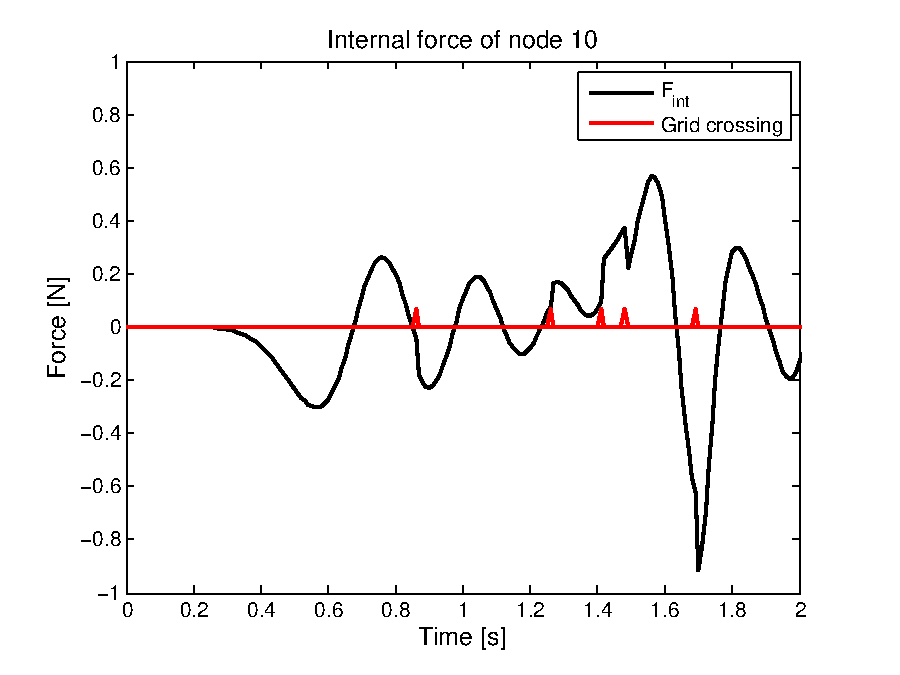
\includegraphics[width=0.7\paperwidth,height=0.7\paperheight]{images/Grid_crossing}
\end{frame}

%--------------------------------------------------------------------------------------------------------------------
\begin{frame}{Grid crossing: vibrating bar}
\begin{overlayarea}{\textwidth}{6cm}
\begin{center}
\only<1>{
\begin{figure}
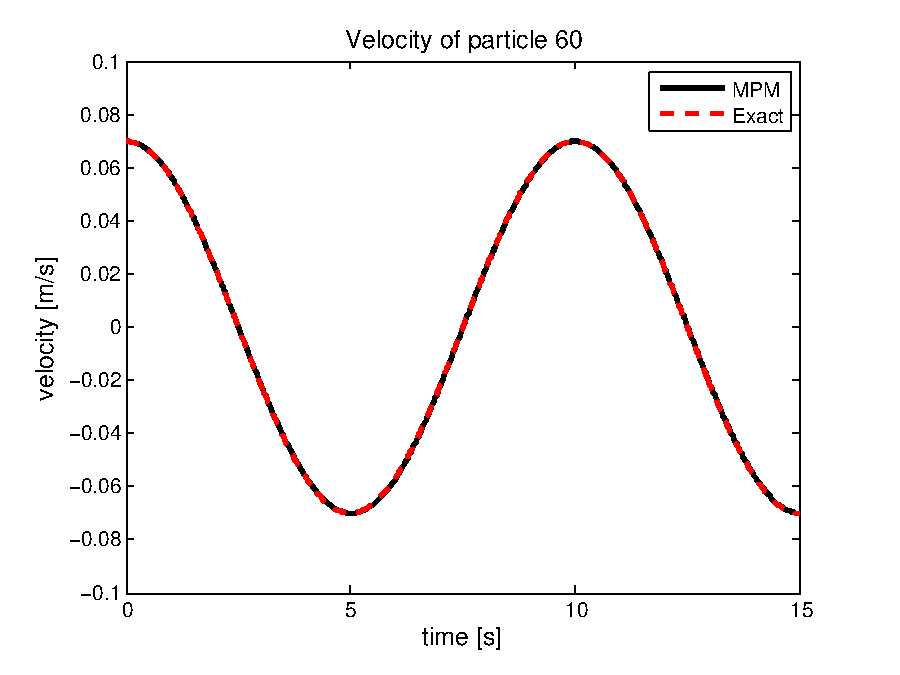
\includegraphics[scale=0.5]{images/vs_vel30}
\caption{\small{No grid crossing (30 elements).}}
\end{figure}
}
\only<2>{
\begin{figure}
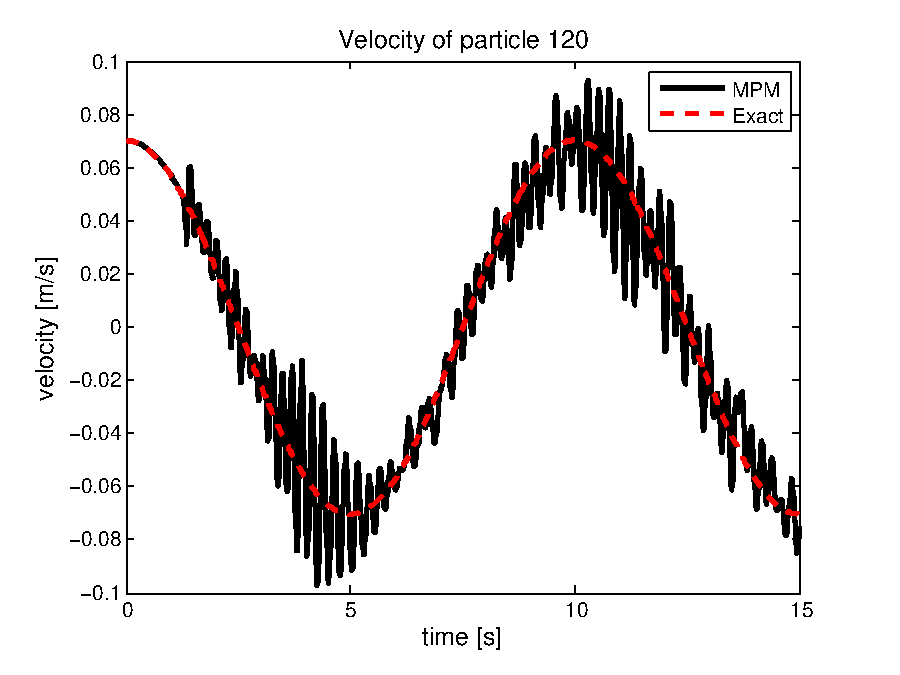
\includegraphics[scale=0.5]{images/vs_vel60}
\caption{\small{Grid crossing (60 elements).}}
\end{figure}
}
\end{center}
\end{overlayarea}
\end{frame}


%--------------------------------------------------------------------------------------------------------------------
\begin{frame}{Grid crossing: oedometer}

\end{frame}
%--------------------------------------------------------------------------------------------------------------------

\begin{frame}{Error versus number of elements}
\begin{table}
\centering
 \begin{tabular}{c | c c c}
   & FEM & MPM(1) & MPM(4)\\
   \hline
  4  & $5.3698 \cdot 10^{-4}$ & $1.2918 \cdot 10^{-3}$ & $1.0374 \cdot 10^{-3}$ \\
  8  & $1.3456 \cdot 10^{-4}$ & $3.2595 \cdot 10^{-4}$ & $2.6167 \cdot 10^{-4}$ \\
  16 & $3.3657 \cdot 10^{-5}$ & $8.1795 \cdot 10^{-5}$ & $6.5694 \cdot 10^{-5}$ \\
  32 & $8.4138 \cdot 10^{-6}$ & $2.0632 \cdot 10^{-5}$ & $1.6625 \cdot 10^{-5}$ \\
  64 & $2.1019 \cdot 10^{-6}$ & $5.4969 \cdot 10^{-6}$ & $4.5505 \cdot 10^{-6}$ \\
 \end{tabular}
 \caption{Vibrating bar: RMS Error versus number of elements.}
\end{table}
\pause
\begin{tcolorbox}[colback=blue!5,colframe=blue!40!black,title=Order of accuracy]
All three methods are second order accurate.
\end{tcolorbox}
 
\end{frame}
%---------------------------------------------------------------------------------------------------------------------
\begin{frame}{Accuracy: vibrating bar}
\begin{tikzpicture}
% \begin{semilogyaxis}[ 
% xlabel={number of elements}, 
% ylabel={RMS Error} 
% ] 

\begin{axis}[
        %height=0.5\textwidth,
        %width=\textwidth,
        xlabel=number of elements,
        xmode=log,
        log basis x={2},
        xtick = {4,8,16,32,64},
        xticklabels={2,3,4,5,6},
        ylabel=RMS error,
        ymode=log,
        log basis y={2},
%         ytick = {2^{-9},2e-11,2e-13,2e-15,2e-15,2e-17,2e-19},
%         yticklabels={-9,-11,-13,-15,-17,-19}
]
\addplot coordinates { 
  (4,  5.3698e-04) 
  (8,  1.3456e-04)
  (16, 3.3657e-05)
  (32, 8.4138e-06)
  (64, 2.1019e-06)
  };

\addplot coordinates { 
  (4,  1.2918e-03) 
  (8,  3.2595 e-04)
  (16, 8.1795e-05)
  (32, 2.0632e-05)
  (64, 5.4969e-06)
  };
  
\addplot[color=black,mark=triangle*] coordinates { 
  (4,  1.0374e-03) 
  (8,  2.6167e-04)
  (16, 6.5694e-05)
  (32, 1.6625e-05)
  (64, 4.5505e-06)
  };  
\legend{FEM, MPM(1), MPM(4)} 
\end{axis}
%\end{semilogyaxis} 
\end{tikzpicture}
\end{frame}

\end{document}
\grid
